\documentclass[lettersize,journal]{IEEEtran}
\usepackage{amsmath,amsfonts}
\usepackage{tikz}
\usetikzlibrary{calc}
\usepackage{xparse,amssymb}

\begin{document}

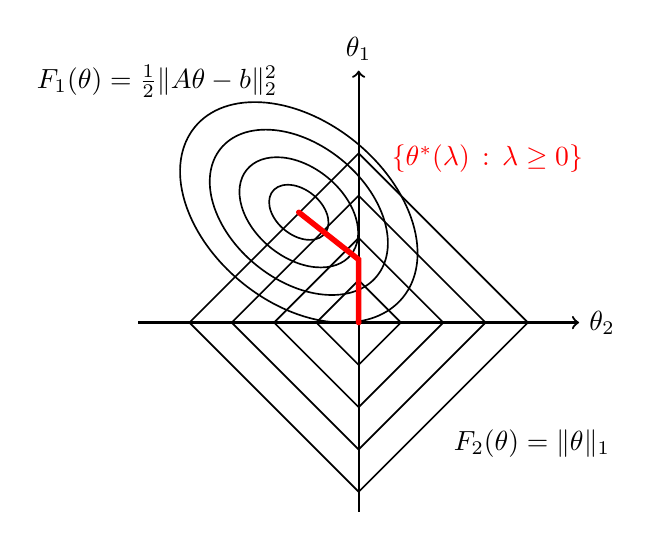
\begin{tikzpicture}[scale=0.4] % Adjust the scale factor as needed

    % Square 1
    % Square 2
    \draw[rotate=45, line width=0.6pt] (-0.95, -0.95) rectangle (0.95, 0.95)node[label={[label distance=-2.5cm, xshift=2.2cm]above:\textcolor{black}{$F_2(\theta) = \lVert \theta \rVert_1$}}] {};

    % Square 3

    % Square 4
    \draw[rotate=-45, line width=0.6pt] (-1.9, -1.9) rectangle (1.9, 1.9);

    % Square 5

    % Square 6
    \draw[rotate=-45, line width=0.6pt] (-2.85, -2.85) rectangle (2.85, 2.85);

    % Square 7

    % Square 8
    \draw[rotate=-45, line width=0.6pt] (-3.8, -3.8) rectangle (3.8, 3.8);


    % Axes
    \draw[->, line width=0.8pt] (-7, 0) -- (7, 0) node[right] {$\theta_2$};
    \draw[->, line width=0.8pt] (0, -6) -- (0, 8) node[above] {$\theta_1$};

    \begin{scope}[xslant=-0.4]
        % Contour 1

        % Contour 2
        \draw[line width=0.6pt] (-0.5, 3.5) circle (0.875);

        % Contour 3

        \draw[line width=0.6pt] (-0.5, 3.5) circle (1.75)  node[label={[above=1.2cm, xshift=-1.8cm]above:\textcolor{black}{$F_1(\theta) = \frac{1}{2}\lVert A \theta - b \rVert_2^2 $}}] {};

        % Contour 2

        % Contour 3
        \draw[line width=0.6pt] (-0.5, 3.5) circle (2.625) ;
        % Contour 3

        % Contour 3
        \draw[line width=0.6pt] (-0.5, 3.5) circle (3.5) ;

        % Intersection points
        \coordinate (ellipseIntersection) at (-0.5, 3.5);
        \coordinate (squareIntersection) at (0, 0);

        % Draw the red line through the tangential points
        \draw[red, line width=2.0pt ] (ellipseIntersection) -- node[above right = 0.65cm, red] {$\left\lbrace \theta^*(\lambda) \, : \, \lambda \ge 0 \right\rbrace $} (0.8, 2) -- (squareIntersection);

    \end{scope}

    \draw[red, fill=red] (0,0) circle (.07);
    \draw[red, fill=red] (-1.9, 3.5) circle (.07);

\end{tikzpicture}

\end{document}